\documentclass[10pt,twocolumn]{article}

\usepackage[a4paper,margin=17mm,columnsep=7mm]{geometry}
\usepackage[T1]{fontenc}
\usepackage{lmodern}
\usepackage{microtype}
\usepackage{amsmath,amssymb,bm}
\usepackage{booktabs,tabularx,array}
\usepackage{enumitem}
\usepackage{xcolor}
\usepackage{tikz}
\usetikzlibrary{arrows.meta,positioning,fit,calc,shapes.geometric,backgrounds,matrix}
\usepackage{pgfplots}
\pgfplotsset{compat=1.18}
\usepackage{hyperref}
\usepackage[capitalise,noabbrev]{cleveref}

\definecolor{airbusblue}{HTML}{0B5FA5}
\definecolor{airbuscyan}{HTML}{00A6C8}
\definecolor{navy}{HTML}{071D3B}
\definecolor{softblue}{HTML}{EAF5F8}
\definecolor{softgray}{HTML}{F2F5F7}
\definecolor{resultgreen}{HTML}{15866D}
\definecolor{warningorange}{HTML}{D98716}

\hypersetup{
  colorlinks=true,
  linkcolor=airbusblue,
  citecolor=airbusblue,
  urlcolor=airbusblue,
  pdftitle={A Block-Encoded Carleman-Lattice Boltzmann Solver for the Convecting Taylor-Green Vortex},
  pdfauthor={Syed Mohaiminul Hoque}
}

\setlist[itemize]{leftmargin=*,nosep}
\setlength{\parindent}{1em}
\setlength{\parskip}{0.15em}
\renewcommand{\arraystretch}{1.12}

\newcommand{\Rey}{\mathrm{Re}}
\newcommand{\TTS}{\mathrm{TTS}}
\newcommand{\vect}[1]{\bm{#1}}
\newcommand{\email}[1]{\href{mailto:#1}{\texttt{#1}}}

\title{\vspace{-1.1em}\textbf{A Block-Encoded Carleman-Lattice Boltzmann Solver\\
for the Convecting Taylor-Green Vortex}\\[-0.1em]
\large Concept Proposal for the Airbus Global Quantum + AI Challenge 2026}
\author{Syed Mohaiminul Hoque\\
\normalsize Team Quantum Aero Solver\\
\normalsize \email{syedmuhaimintahsin@gmail.com}}
\date{4 September 2026}

\begin{document}
\maketitle

\begin{abstract}
Accurate aerodynamic prediction requires solving nonlinear, dissipative partial
differential equations at resolutions whose computational and memory costs grow
rapidly with Reynolds number. This paper proposes a fault-tolerant quantum
algorithm for the two-dimensional convecting Taylor-Green vortex based on a
D2Q9 lattice Boltzmann discretization, Carleman linearization of the nonlinear
BGK collision, unitary block encoding of the resulting non-unitary map, and
reversible periodic streaming. The benchmark is separated into a periodic box
length $L_{\mathrm{box}}=2\pi$ and vortex scale $L_c=1$ to remove an ambiguity
in the challenge statement. Preliminary implementation validates a local
90-dimensional lifted collision through an eight-qubit unitary dilation with
maximum block error $6.94\times10^{-17}$ and maximum unitarity error
$5.11\times10^{-15}$. A full spatial collision-streaming comparison gives
velocity relative $L_2$ error $1.28\times10^{-5}$ between the Carleman and exact
BGK paths for a small test. The measured dense routed synthesis is expensive,
and the raw post-selection probability is only $1.77\%$; these results define
the optimization target rather than establish advantage. We therefore specify
an end-to-end, fixed-accuracy protocol that includes preparation, amplification,
routing, fault tolerance, and observable extraction. The target claim is a
bounded advantage for selected observables, not full-field recovery.
\end{abstract}

\noindent\textbf{Keywords:} quantum computational fluid dynamics, lattice
Boltzmann method, Carleman linearization, block encoding, Taylor-Green vortex,
fault-tolerant quantum computing.

\section{Motivation and Objective}
Airbus identifies predictive aerodynamics as a high-value computational
capability because extreme operating conditions remain costly to reproduce in
physical tests and expensive to resolve numerically \cite{airbus2026}. The
challenge asks participants to simulate the convecting Taylor-Green vortex and
quantify how runtime, memory or qubits, and numerical error scale with Reynolds
number. The exact solution makes this problem unusually suitable for separating
physical fidelity from circuit executability.

The proposed method follows the fault-tolerant quantum computing (FTQC) and
lattice Boltzmann route. Its research question is:

\begin{quote}
Can a structured block encoding of collision, combined with logarithmic-size
position registers and unitary streaming, reduce time-to-solution or memory for
selected flow observables at a fixed physical error as $\Rey$ increases?
\end{quote}

This is intentionally narrower than claiming exponential advantage for an
entire velocity field. Recent end-to-end analysis shows that Carleman
convergence, time stepping, conditioning, and data extraction can eliminate
nominal quantum speedups \cite{jennings2025}. The proposed experiments measure
each of these costs and include a no-go decision if no crossover survives.

\section{Benchmark Definition}
\subsection{Governing equations}
For velocity $\vect{u}=(u,v)$, pressure $p$, density $\rho$, and kinematic
viscosity $\nu$, the two-dimensional incompressible Navier-Stokes equations are
\begin{align}
  \nabla\cdot\vect{u} &= 0, \label{eq:continuity}\\
  \partial_t\vect{u}+(\vect{u}\cdot\nabla)\vect{u}
  &= -\rho^{-1}\nabla p+\nu\nabla^2\vect{u}. \label{eq:momentum}
\end{align}
The exact convecting Taylor-Green solution is
\begin{align}
u(x,y,t) &= U_c + V_0\sin\xi\cos\eta\,A(t),\label{eq:exactu}\\
v(x,y,t) &= V_c - V_0\cos\xi\sin\eta\,A(t),\label{eq:exactv}\\
p(x,y,t) &= p_0+\frac{\rho V_0^2}{4}
 \left[\cos(2\xi)+\cos(2\eta)\right]A(t)^2,\label{eq:exactp}
\end{align}
where
\begin{align}
\xi&=\frac{x-U_ct}{L_c}, &
\eta&=\frac{y-V_ct}{L_c},\nonumber\\
A(t)&=\exp\left(-\frac{2\nu t}{L_c^2}\right).&&
\end{align}
We use
\begin{align}
L_{\mathrm{box}}&=2\pi, & L_c&=1, & V_0=U_c=\rho&=1,\nonumber\\
V_c&=p_0=0, & \nu&=\frac{V_0L_c}{\Rey}.&&
\end{align}
This distinction is essential: using $L=2\pi$ simultaneously as the domain
length and trigonometric scale makes the stated field non-periodic. The final
submission will record the convention in every dataset and request organizer
confirmation.

\subsection{Accuracy metrics}
The primary error is the relative velocity-field norm
\begin{equation}
\epsilon_{L_2}(t)=
\frac{\left\|\vect{u}_{\mathrm{sim}}(t)-\vect{u}_{\mathrm{exact}}(t)\right\|_2}
{\left\|\vect{u}_{\mathrm{exact}}(t)\right\|_2}.
\label{eq:l2}
\end{equation}
Because the uniform streamwise component can dilute the vortex error, we also
report the same norm after subtracting $(U_c,V_c)$. The kinetic energy is
\begin{equation}
K(t)=\frac{1}{2}\left\langle u^2+v^2\right\rangle.
\label{eq:ke}
\end{equation}
Mass drift, momentum drift, and $\|\nabla\cdot\vect{u}\|_2$ complete the
physical diagnostics.

\begin{figure*}[t]
\centering
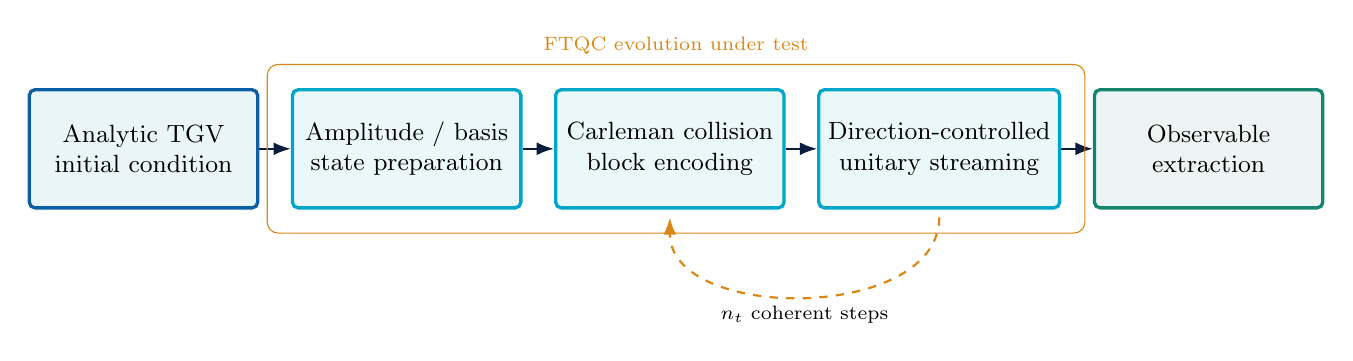
\begin{tikzpicture}[
  node distance=5mm and 4mm,
  stage/.style={draw=airbusblue, rounded corners=2pt, very thick,
    minimum width=29mm, minimum height=15mm, align=center, fill=softblue,
    font=\small},
  quantum/.style={stage,draw=airbuscyan,fill=airbuscyan!8},
  check/.style={stage,draw=resultgreen,fill=resultgreen!8},
  arrow/.style={-{Latex[length=2.2mm]},thick,draw=navy},
  loop/.style={-{Latex[length=2.2mm]},thick,dashed,draw=warningorange}
]
\node[stage] (init) {Analytic TGV\\initial condition};
\node[quantum,right=of init] (encode) {Amplitude / basis\\state preparation};
\node[quantum,right=of encode] (collide) {Carleman collision\\block encoding};
\node[quantum,right=of collide] (stream) {Direction-controlled\\unitary streaming};
\node[check,right=of stream] (measure) {Observable\\extraction};
\draw[arrow] (init) -- (encode);
\draw[arrow] (encode) -- (collide);
\draw[arrow] (collide) -- (stream);
\draw[arrow] (stream) -- (measure);
\draw[loop] ($(stream.south)+(0,-1mm)$) to[out=-90,in=-90]
 node[below,font=\scriptsize] {$n_t$ coherent steps} ($(collide.south)+(0,-1mm)$);
\node[draw=warningorange,rounded corners,fit=(encode)(collide)(stream),
 inner sep=3mm,label={[font=\scriptsize,text=warningorange]above:FTQC evolution under test}] {};
\end{tikzpicture}
\caption{Proposed end-to-end method. The claimed quantum path must keep the
lifted state coherent between collision and streaming; classical re-lifting is
allowed only in validation experiments, not in the advantage claim.}
\label{fig:pipeline}
\end{figure*}

\section{Classical D2Q9 Foundation}
The classical and quantum paths use the same D2Q9 finite-velocity model so that
the initial comparison does not mix algorithmic and discretization errors. The
velocities and weights are
\begin{align}
\vect{e}_i &\in \{(0,0),(\pm1,0),(0,\pm1),(\pm1,\pm1)\},\\
w_0&=\frac49,\qquad w_{1:4}=\frac19,\qquad w_{5:8}=\frac1{36},
\qquad c_s^2=\frac13.
\end{align}
Macroscopic fields are reconstructed by
\begin{equation}
\rho=\sum_{i=0}^{8}f_i,\qquad
\rho\vect{u}=\sum_{i=0}^{8}f_i\vect{e}_i.
\end{equation}
The second-order equilibrium is
\begin{equation}
f_i^{\mathrm{eq}}=w_i\rho\left[
1+\frac{\vect{e}_i\cdot\vect{u}}{c_s^2}
+\frac{(\vect{e}_i\cdot\vect{u})^2}{2c_s^4}
-\frac{\vect{u}\cdot\vect{u}}{2c_s^2}\right],
\label{eq:feq}
\end{equation}
followed by BGK collision and periodic streaming,
\begin{align}
f_i^{\star}(\vect{x},t)&=f_i(\vect{x},t)
-\omega\left(f_i-f_i^{\mathrm{eq}}\right),\label{eq:bgk}\\
f_i(\vect{x}+\vect{e}_i,t+\Delta t)&=f_i^{\star}(\vect{x},t),
\qquad \omega=\tau^{-1}.\label{eq:stream}
\end{align}

\begin{figure}[t]
\centering
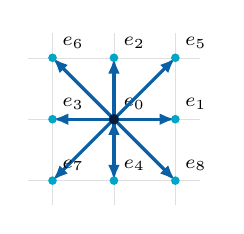
\begin{tikzpicture}[scale=0.78]
  \draw[step=1cm,gray!25,very thin] (-1.4,-1.4) grid (1.4,1.4);
  \foreach \x/\y/\lab in {
    0/0/0,1/0/1,0/1/2,-1/0/3,0/-1/4,
    1/1/5,-1/1/6,-1/-1/7,1/-1/8}
  {
    \draw[-{Latex[length=2mm]},very thick,airbusblue] (0,0) -- (\x,\y);
    \fill[airbuscyan] (\x,\y) circle (2pt);
    \node[font=\scriptsize,anchor=south west] at (\x,\y) {$e_{\lab}$};
  }
  \fill[navy] (0,0) circle (2.4pt);
\end{tikzpicture}
\caption{D2Q9 velocity stencil used by both solver paths. Streaming is a
permutation and is therefore naturally unitary on a periodic grid.}
\label{fig:d2q9}
\end{figure}

The in-repository BGK implementation is a controlled baseline, not a
state-of-the-art comparator. A Fourier pseudo-spectral or high-order
finite-volume solver will be added before final advantage assessment.

\section{Quantum Collision and Streaming}
\subsection{Carleman linearization}
Near reference density $\rho_0$, \,\cref{eq:feq} is expressed as
\begin{equation}
\vect{f}^{\mathrm{eq}}\approx L\vect{f}
+Q:(\vect{f}\otimes\vect{f}),
\end{equation}
where $L\in\mathbb{R}^{9\times9}$ and
$Q\in\mathbb{R}^{9\times9\times9}$. Define
\begin{equation}
\vect{z}=\begin{bmatrix}\vect{f}\\
\vect{f}\otimes\vect{f}\end{bmatrix}\in\mathbb{R}^{90},
\qquad
R=(1-\omega)I+\omega L.
\end{equation}
At order two, the collision is approximated by the linear recurrence
\begin{equation}
\vect{z}^{\star}=M\vect{z},\qquad
M=
\begin{bmatrix}
R & \omega Q\\
0 & R\otimes R
\end{bmatrix}.
\label{eq:carleman}
\end{equation}
Here $Q$ in the upper-right block denotes the matricized contraction from 81 to
9 components. General convergence of Carleman truncation is conditional;
dissipative quadratic systems require explicit parameter bounds and cannot be
assumed efficient for arbitrary flow regimes \cite{liu2021}.

\subsection{Unitary dilation and success probability}
Let $\alpha\geq\|M\|_2$ and $A=M/\alpha$. Padding the system dimension from 90
to 128 permits an eight-qubit unitary dilation
\begin{equation}
U_A=
\begin{bmatrix}
A & \sqrt{I-AA^{\dagger}}\\
\sqrt{I-A^{\dagger}A} & -A^{\dagger}
\end{bmatrix}.
\label{eq:dilation}
\end{equation}
Post-selecting the signal ancilla in $\lvert 0\rangle$ applies $A$ to the system
register. The measured success probability for the current test state is
\begin{equation}
p_{\mathrm{succ}}=
\frac{\|M\vect{z}\|_2^2}{\alpha^2\|\vect{z}\|_2^2}=0.01774,
\end{equation}
which implies about $1/p_{\mathrm{succ}}=56.4$ raw attempts or an amplitude
amplification scale $1/\sqrt{p_{\mathrm{succ}}}=7.51$. These factors are part of
the resource model. QSVT and oblivious amplitude amplification provide the
mathematical framework for replacing dense dilation with structured block
encodings \cite{gilyen2019}.

\begin{figure}[t]
\centering
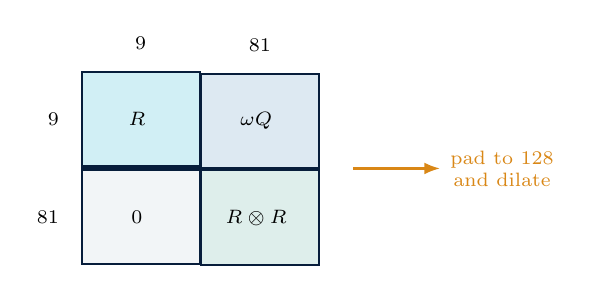
\begin{tikzpicture}[
  block/.style={draw=navy,thick,minimum width=15mm,minimum height=12mm,
    align=center,font=\scriptsize},
  label/.style={font=\scriptsize,align=center}
]
\matrix[matrix of nodes,nodes={block},row sep=-\pgflinewidth,column sep=-\pgflinewidth] (m) {
  |[fill=airbuscyan!18]| $R$ & |[fill=airbusblue!14]| $\omega Q$ \\
  |[fill=softgray]| $0$ & |[fill=resultgreen!14]| $R\otimes R$ \\
};
\node[label,above=1.5mm of m-1-1] {$9$};
\node[label,above=1.5mm of m-1-2] {$81$};
\node[label,left=1.5mm of m-1-1] {$9$};
\node[label,left=1.5mm of m-2-1] {$81$};
\draw[-{Latex[length=2mm]},warningorange,thick]
  ($(m.east)+(3mm,0)$) -- ++(11mm,0)
  node[right,label] {pad to 128\\and dilate};
\end{tikzpicture}
\caption{Structure of the 90-dimensional local order-two Carleman collision.
The production objective is to compile this structure rather than synthesize a
generic dense $256\times256$ unitary.}
\label{fig:carlemanblock}
\end{figure}

\subsection{Coherent streaming and extraction}
For a periodic $N_x\times N_y$ grid, the position registers require
$\lceil\log_2N_x\rceil+\lceil\log_2N_y\rceil$ qubits. Direction-controlled
modular addition implements \,\cref{eq:stream} as a permutation. The primary
outputs are $K(t)$ and selected Fourier coefficients. Full-field tomography is
not included in the claimed advantage route because its output cost grows with
the number of degrees of freedom.

The current spatial validator reconstructs
$\vect{f}\otimes\vect{f}$ classically between timesteps. This is useful for
physics validation but is not an end-to-end quantum algorithm. The central
research milestone is a coherent local/global lift or an alternative
incompressible-LBM construction that preserves a bounded advantage
\cite{jennings2025,zamora2026}.

\section{Preliminary Results}
\subsection{Corrected classical datasets}
The legacy datasets used the inconsistent length convention and produced
approximately 25--33\% relative error. They were regenerated with
$L_{\mathrm{box}}=2\pi$, $L_c=1$, and $t=1$. Final errors now lie between
$4.43\times10^{-3}$ and $4.63\times10^{-3}$ for the configured scaling points.

\begin{table}[t]
\centering
\caption{Measured corrected classical scaling points at $t=1$. The
$\Rey=5000$ row is an under-resolved pilot, not a production result.}
\label{tab:sweep}
\small
\begin{tabular}{rrrrr}
\toprule
$\Rey$ & $N$ & Steps & Runtime (s) & $\epsilon_{L_2}$\\
\midrule
10   & 32  & 395  & 0.86   & 0.004635\\
100  & 64  & 789  & 4.53   & 0.004432\\
400  & 128 & 1578 & 51.99  & 0.004497\\
1000 & 256 & 3156 & 509.83 & 0.004526\\
5000 & 128 & 1578 & 65.50  & 0.004533$^{\ast}$\\
\bottomrule
\multicolumn{5}{l}{\scriptsize $^{\ast}$Measured pilot; grid convergence not established.}
\end{tabular}
\end{table}

\begin{figure*}[t]
\centering
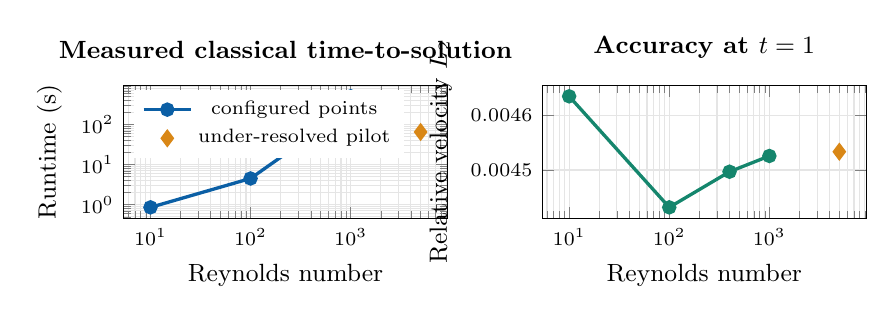
\begin{tikzpicture}
\begin{axis}[
  name=runtime,width=0.47\textwidth,height=0.27\textwidth,
  xmode=log,ymode=log,xlabel={Reynolds number},ylabel={Runtime (s)},
  title={Measured classical time-to-solution},grid=both,
  grid style={gray!20},tick label style={font=\scriptsize},
  label style={font=\small},title style={font=\small\bfseries},
  legend style={font=\scriptsize,draw=none,at={(0.03,0.97)},anchor=north west}
]
\addplot[airbusblue,very thick,mark=*] coordinates
  {(10,0.8602) (100,4.5310) (400,51.9919) (1000,509.8260)};
\addlegendentry{configured points}
\addplot[warningorange,only marks,mark=diamond*,mark size=3pt]
  coordinates {(5000,65.5005)};
\addlegendentry{under-resolved pilot}
\end{axis}
\begin{axis}[
  at={($(runtime.east)+(12mm,0)$)},anchor=west,
  width=0.47\textwidth,height=0.27\textwidth,
  xmode=log,xlabel={Reynolds number},ylabel={Relative velocity $L_2$},
  title={Accuracy at $t=1$},grid=both,
  grid style={gray!20},tick label style={font=\scriptsize},
  label style={font=\small},title style={font=\small\bfseries},
  scaled y ticks=false,yticklabel style={/pgf/number format/fixed,/pgf/number format/precision=5}
]
\addplot[resultgreen,very thick,mark=*] coordinates
  {(10,0.00463495) (100,0.00443167) (400,0.00449691) (1000,0.00452572)};
\addplot[warningorange,only marks,mark=diamond*,mark size=3pt]
  coordinates {(5000,0.00453349)};
\end{axis}
\end{tikzpicture}
\caption{Directly measured corrected sweep. Runtime values are machine-specific
and presently have one repetition; final submission points will use warmups,
at least five repetitions, and confidence intervals.}
\label{fig:scaling}
\end{figure*}

\subsection{Collision, circuit, and noise evidence}
The local block encoding reproduces the 90-dimensional collision with maximum
amplitude error $6.94\times10^{-17}$, and \,\cref{eq:dilation} is unitary to
$5.11\times10^{-15}$. A full spatial comparison at
$(\Rey,N,t)=(100,32,0.1)$ gives Carleman-versus-exact-BGK relative errors
$1.28\times10^{-5}$ in velocity and $2.21\times10^{-7}$ in populations.

The corrected streaming noise experiment transpiles to the $\{u,\mathrm{CX}\}$
basis and actually passes a depolarizing noise model to Aer. With 20,000 shots,
one-qubit error $10^{-3}$, and two-qubit error $10^{-2}$, the noisy-versus-ideal
Hellinger fidelity is 0.964 and the total variation distance is 0.036.

\begin{table}[t]
\centering
\caption{Connectivity-aware resource proxy for the complete local dense
collision dilation on an eight-qubit bidirectional ring.}
\label{tab:resources}
\small
\begin{tabular}{lr}
\toprule
Resource & Measured value\\
\midrule
Transpiled depth & 107,128\\
Single-qubit $u$ gates & 51,483\\
CX gates & 87,216\\
Raw post-selection probability & 0.01774\\
Expected raw attempts & 56.4\\
Amplitude amplification scale & 7.51\\
\bottomrule
\end{tabular}
\end{table}

These counts include routing but exclude arbitrary-rotation synthesis into
Clifford+$T$, error correction, and magic-state factories. They are a dense
upper bound, not a favorable resource claim.

\section{Experimental Program}
The experiments are designed around fixed physical accuracy, not fixed grid
size. Each configuration records code revision, seeds, precision, dependency
versions, processor or backend, transpiler settings, raw counts, and wall-clock
protocol.

\begin{table*}[t]
\centering
\caption{Planned experiments and decision criteria.}
\label{tab:plan}
\small
\begin{tabularx}{\textwidth}{p{0.18\textwidth}p{0.27\textwidth}X p{0.21\textwidth}}
\toprule
Work package & Sweep & Recorded outputs & Pass criterion\\
\midrule
Physics convergence & $\Rey=10,100,400,1000,2000,5000$; $N=32$--2048;
$\mathrm{Ma}=0.1$--0.0125 & Total/vortex $L_2$, energy, phase, mass,
momentum, divergence & Grid and Mach convergence at $t=1$\\
Collision fidelity & Carleman order 1--3; 1--1000 steps; density and velocity
perturbations & Population and observable drift versus exact BGK & Truncation
error fits declared budget\\
Quantum correctness & 1, 2, 5, 10, and 50 coherent timesteps & State and
observable error, success probability & No classical operation in claimed path\\
Noise sensitivity & Gate error $10^{-4}$--$10^{-2}$; shots $10^3$--$10^6$ &
Fidelity, bias, variance, confidence interval & Noise applied after compilation\\
Resource scaling & $N=8$--2048, $\Rey=10$--5000,
$\epsilon=10^{-1}$--$10^{-4}$ & Logical/physical qubits, $T$ count/depth,
block calls, shots, runtime & Complete cost ledger\\
Classical comparison & BGK plus spectral or high-order finite volume & Runtime,
peak memory, accuracy & Same physics, observable, and tolerance\\
\bottomrule
\end{tabularx}
\end{table*}

The required final plots are: (i) time-to-solution versus $\Rey$ at fixed
$\epsilon$, (ii) memory or physical qubits versus $\Rey$, (iii) $L_2$ and
kinetic-energy error versus $\Rey$, and (iv) a stacked cost decomposition for
preparation, collision, streaming, amplification, and measurement.

\section{End-to-End Advantage Test}
A compact state representation does not prove an advantage. For one declared
observable and error tolerance $\epsilon$, total quantum time is modeled as
\begin{align}
T_Q(\epsilon,\Rey)={}&T_{\mathrm{prep}}
+n_t\left[N_{\mathrm{BE}}C_{\mathrm{AA}}(p)+N_S\right]\nonumber\\
&\times t_{\mathrm{cycle}}+N_{\mathrm{shots}}T_{\mathrm{meas}}.
\label{eq:cost}
\end{align}
Here $N_{\mathrm{BE}}$ is block-encoding cost,
$C_{\mathrm{AA}}(p)$ is amplification overhead, $N_S$ is streaming cost, and
$N_{\mathrm{shots}}$ follows from the observable precision. The logical cycle
time includes routing, rotation synthesis, code distance, magic-state factory
throughput, and a declared failure probability.

\begin{figure}[t]
\centering
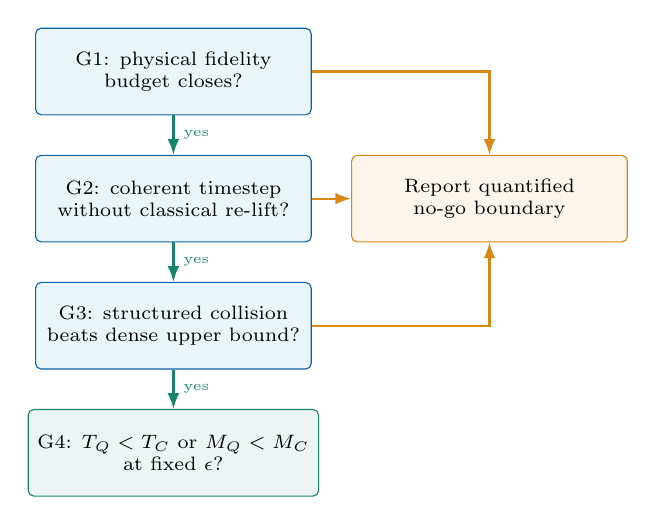
\begin{tikzpicture}[
  gate/.style={draw,rounded corners=2pt,minimum width=35mm,minimum height=11mm,
    align=center,font=\scriptsize},
  yes/.style={-{Latex[length=2mm]},thick,resultgreen},
  no/.style={-{Latex[length=2mm]},thick,warningorange}
]
\node[gate,draw=airbusblue,fill=softblue] (g1) {G1: physical fidelity\\budget closes?};
\node[gate,draw=airbusblue,fill=softblue,below=5mm of g1] (g2) {G2: coherent timestep\\without classical re-lift?};
\node[gate,draw=airbusblue,fill=softblue,below=5mm of g2] (g3) {G3: structured collision\\beats dense upper bound?};
\node[gate,draw=resultgreen,fill=resultgreen!8,below=5mm of g3] (g4) {G4: $T_Q<T_C$ or $M_Q<M_C$\\at fixed $\epsilon$?};
\node[gate,draw=warningorange,fill=warningorange!8,right=5mm of g2] (nogo) {Report quantified\\no-go boundary};
\draw[yes] (g1) -- node[right,font=\tiny] {yes} (g2);
\draw[yes] (g2) -- node[right,font=\tiny] {yes} (g3);
\draw[yes] (g3) -- node[right,font=\tiny] {yes} (g4);
\draw[no] (g1.east) -| (nogo.north);
\draw[no] (g2.east) -- (nogo.west);
\draw[no] (g3.east) -| (nogo.south);
\end{tikzpicture}
\caption{Evidence gates for accepting or rejecting a bounded advantage claim.
Failure is reported as a quantified no-go result rather than hidden.}
\label{fig:gates}
\end{figure}

The claim is accepted only when total time or memory is lower than both
classical comparators at the same $(\Rey,t,\epsilon)$ for the same observable.
Three hardware levels will be reported: ideal logical all-to-all, routed logical
nearest-neighbor, and fault tolerant with physical qubits and wall time.

\section{Risks and Mitigations}
\begin{table*}[t]
\centering
\caption{Principal technical risks.}
\label{tab:risks}
\small
\begin{tabularx}{\textwidth}{p{0.25\textwidth}p{0.15\textwidth}X}
\toprule
Risk & Likelihood / impact & Mitigation\\
\midrule
Carleman truncation fails at high $\Rey$ & High / high & Stability map,
rescaling, adaptive order, and pivot to an end-to-end bounded-advantage
incompressible LBM formulation\\
Post-selection dominates & High / high & Optimize normalization, exploit local
encoding, include amplification, and enforce a stop gate\\
Dense synthesis remains exponential & High / high & Exploit D2Q9 sparsity,
symmetry, repeated coefficients, and local collision reuse\\
Data extraction removes the speedup & High / high & Restrict primary outputs to
kinetic energy and selected modes; account for every sample\\
Classical reference is weak & Medium / high & Add pseudo-spectral or high-order
finite-volume baselines at identical tolerance\\
Benchmark convention is disputed & Medium / medium & Publish both length scales
and obtain organizer confirmation\\
\bottomrule
\end{tabularx}
\end{table*}

\section{Schedule and Deliverables}
The proposed sixteen-week program has six gated phases:
\begin{enumerate}[leftmargin=*,itemsep=1pt]
\item \textbf{Weeks 1--2: benchmark lock.} Complete convergence study,
provenance schema, and independent classical comparator.
\item \textbf{Weeks 3--6: coherent algorithm.} Remove classical re-lifting from
the claimed path and validate several timesteps.
\item \textbf{Weeks 7--10: circuit engineering.} Construct the sparse block
encoding and compile collision plus streaming.
\item \textbf{Weeks 11--13: scale study.} Execute $\Rey$ and accuracy sweeps and
produce fixed-error scaling figures.
\item \textbf{Weeks 14--15: FTQC assessment.} Estimate Clifford+$T$, code
distance, factories, physical qubits, and wall time.
\item \textbf{Week 16: submission.} Deliver the paper, source, code, corrected
datasets, raw results, and independent rerun checklist.
\end{enumerate}

\section{Expected Contribution}
The project is designed to produce a scientifically useful result in either
direction. A successful outcome is a defensible bounded advantage for selected
aerodynamic observables, supported by a complete resource ledger. A negative
outcome is a quantified boundary identifying whether truncation, conditioning,
amplification, synthesis, or readout prevents a crossover. In both cases, the
corrected Taylor-Green benchmark, nine-population collision model, and
reproducibility artifacts provide a foundation for subsequent Airbus
quantum-CFD evaluations.

\section{Conclusion}
This proposal advances beyond a streaming-only or toy-collision demonstration.
It supplies a verified local D2Q9 Carleman collision block, corrected periodic
datasets, full spatial fidelity checks, an applied-noise experiment, and routed
resource evidence. The same evidence also shows why advantage cannot yet be
claimed: dense collision synthesis and low post-selection probability are
costly, and coherent multi-step lifting remains open. The proposed program turns
those limitations into explicit experiments and decision gates. Only an
end-to-end fixed-accuracy crossover for selected observables will be reported as
quantum advantage.

\begin{thebibliography}{99}
\bibitem{airbus2026}
Airbus, ``Quantum Solvers: Enhancing Predictive Aerodynamic Modeling
Capabilities,'' Global Quantum + AI Challenge 2026 Enterprise Challenge
Statement, 2026.

\bibitem{qian1992}
Y. H. Qian, D. d'Humi\`eres, and P. Lallemand, ``Lattice BGK Models for
Navier-Stokes Equation,'' \emph{Europhysics Letters}, vol. 17, no. 6, 1992.

\bibitem{liu2021}
J.-P. Liu, H. \O. Kolden, H. K. Krovi, N. F. Loureiro, K. Trivisa, and
A. M. Childs, ``Efficient quantum algorithm for dissipative nonlinear
differential equations,'' \emph{PNAS}, vol. 118, e2026805118, 2021;
corrected version, arXiv:2011.03185v4, 2026.

\bibitem{gilyen2019}
A. Gily\'en, Y. Su, G. H. Low, and N. Wiebe, ``Quantum singular value
transformation and beyond: exponential improvements for quantum matrix
arithmetics,'' in \emph{Proc. 51st ACM STOC}, pp. 193--204, 2019.

\bibitem{jennings2025}
D. Jennings, K. Korzekwa, M. Lostaglio, R. Ashworth, E. Marsili, and
S. Rolston, ``An end-to-end quantum algorithm for nonlinear fluid dynamics
with bounded quantum advantage,'' arXiv:2512.03758, 2025.

\bibitem{zamora2026}
A. D. Bastida Zamora, L. Budinski, V. Lahtinen, and P. Sagaut, ``Quantum
lattice Boltzmann method for several time steps: A local Carleman linearization
algorithm,'' arXiv:2511.13072v3, 2026.

\bibitem{childs2017}
A. M. Childs, R. Kothari, and R. D. Somma, ``Quantum algorithm for systems of
linear equations with exponentially improved dependence on precision,''
\emph{SIAM Journal on Computing}, vol. 46, no. 6, pp. 1920--1950, 2017.
\end{thebibliography}

\end{document}
